\documentclass{standalone}
\usepackage{tikz}
\usetikzlibrary{patterns, positioning}

\begin{document}
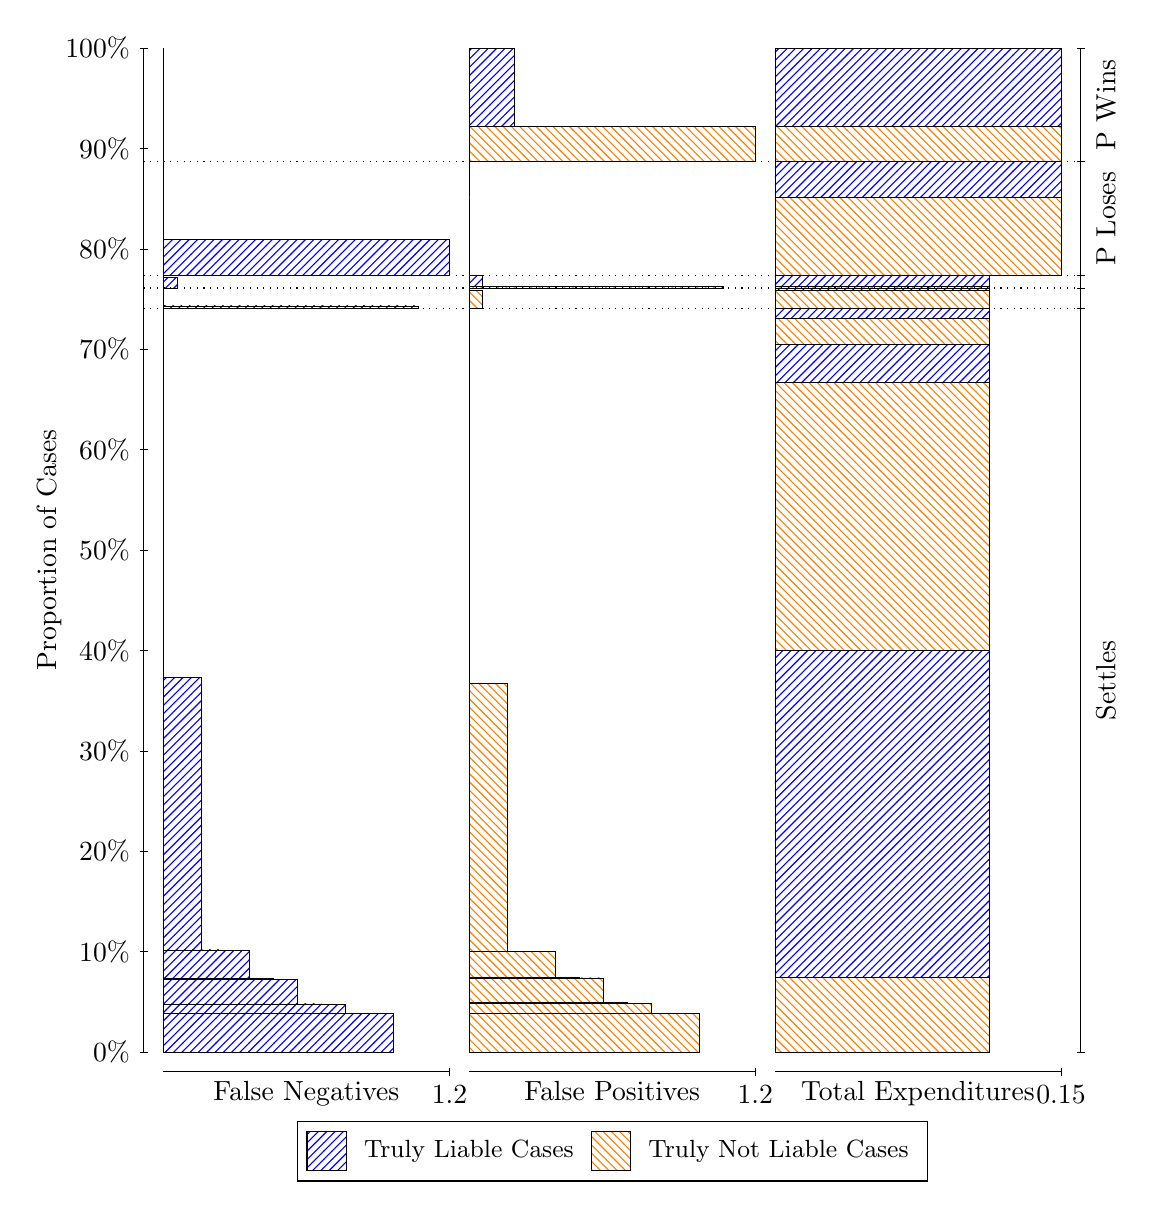
\begin{tikzpicture}
\draw[black, very thin] (1.5,1.75) -- (1.5,14.5);
\node[rotate=90, anchor=center] at (0.3, 8.125) {Proportion of Cases};
\draw[black, very thin] (1.45,1.75) -- (1.55,1.75);
\node[anchor=east] at (1.45, 1.75) {0\%};
\draw[black, very thin] (1.45,3.025) -- (1.55,3.025);
\node[anchor=east] at (1.45, 3.025) {10\%};
\draw[black, very thin] (1.45,4.3) -- (1.55,4.3);
\node[anchor=east] at (1.45, 4.3) {20\%};
\draw[black, very thin] (1.45,5.575) -- (1.55,5.575);
\node[anchor=east] at (1.45, 5.575) {30\%};
\draw[black, very thin] (1.45,6.85) -- (1.55,6.85);
\node[anchor=east] at (1.45, 6.85) {40\%};
\draw[black, very thin] (1.45,8.125) -- (1.55,8.125);
\node[anchor=east] at (1.45, 8.125) {50\%};
\draw[black, very thin] (1.45,9.4) -- (1.55,9.4);
\node[anchor=east] at (1.45, 9.4) {60\%};
\draw[black, very thin] (1.45,10.675) -- (1.55,10.675);
\node[anchor=east] at (1.45, 10.675) {70\%};
\draw[black, very thin] (1.45,11.95) -- (1.55,11.95);
\node[anchor=east] at (1.45, 11.95) {80\%};
\draw[black, very thin] (1.45,13.225) -- (1.55,13.225);
\node[anchor=east] at (1.45, 13.225) {90\%};
\draw[black, very thin] (1.45,14.5) -- (1.55,14.5);
\node[anchor=east] at (1.45, 14.5) {100\%};

\draw[black, very thin] (13.4,1.75) -- (13.4,14.5);
\draw[black, very thin] (13.35,1.75) -- (13.45,1.75);
\node[anchor=west] at (13.35, 1.75) {};
\draw[black, very thin] (13.35,11.194) -- (13.45,11.194);
\node[anchor=west] at (13.35, 11.194) {};
\draw[black, very thin] (13.35,11.453) -- (13.45,11.453);
\node[anchor=west] at (13.35, 11.453) {};
\draw[black, very thin] (13.35,11.614) -- (13.45,11.614);
\node[anchor=west] at (13.35, 11.614) {};
\draw[black, very thin] (13.35,13.057) -- (13.45,13.057);
\node[anchor=west] at (13.35, 13.057) {};
\draw[black, very thin] (13.35,14.5) -- (13.45,14.5);
\node[anchor=west] at (13.35, 14.5) {};

\draw[black, very thin, pattern color=blue, pattern=north east lines] (1.75,1.75) rectangle (4.6758,2.2372);
\draw[black, very thin, pattern color=blue, pattern=north east lines] (1.75,2.2372) rectangle (4.3698,2.2393);
\draw[black, very thin, pattern color=blue, pattern=north east lines] (1.75,2.2393) rectangle (4.0639,2.3574);
\draw[black, very thin, pattern color=blue, pattern=north east lines] (1.75,2.3574) rectangle (3.7579,2.3612);
\draw[black, very thin, pattern color=blue, pattern=north east lines] (1.75,2.3612) rectangle (3.4519,2.6763);
\draw[black, very thin, pattern color=blue, pattern=north east lines] (1.75,2.6763) rectangle (3.146,2.6826);
\draw[black, very thin, pattern color=blue, pattern=north east lines] (1.75,2.6826) rectangle (2.84,3.044);
\draw[black, very thin, pattern color=blue, pattern=north east lines] (1.75,3.044) rectangle (2.534,3.0468);
\draw[black, very thin, pattern color=blue, pattern=north east lines] (1.75,3.0468) rectangle (2.2281,6.5117);
\draw[black, very thin, pattern color=orange, pattern=north west lines] (1.75,6.5117) rectangle (1.75,11.194);
\draw[black, very thin, pattern color=blue, pattern=north east lines] (1.75,11.194) rectangle (4.9818,11.225);
\draw[black, very thin, pattern color=orange, pattern=north west lines] (1.75,11.225) rectangle (1.75,11.453);
\draw[black, very thin, pattern color=blue, pattern=north east lines] (1.75,11.453) rectangle (1.9221,11.592);
\draw[black, very thin, pattern color=orange, pattern=north west lines] (1.75,11.592) rectangle (1.75,11.614);
\draw[black, very thin, pattern color=blue, pattern=north east lines] (1.75,11.614) rectangle (5.3833,12.066);
\draw[black, very thin, pattern color=orange, pattern=north west lines] (1.75,12.066) rectangle (1.75,13.057);
\draw[black, very thin, pattern color=orange, pattern=north west lines] (1.75,13.057) rectangle (1.75,13.509);
\draw[black, very thin, pattern color=blue, pattern=north east lines] (1.75,13.509) rectangle (1.75,14.5);
\draw[black, very thin, pattern color=orange, pattern=north west lines] (5.6333,1.75) rectangle (8.5591,2.239);
\draw[black, very thin, pattern color=orange, pattern=north west lines] (5.6333,2.239) rectangle (8.2532,2.242);
\draw[black, very thin, pattern color=orange, pattern=north west lines] (5.6333,2.242) rectangle (7.9472,2.3708);
\draw[black, very thin, pattern color=orange, pattern=north west lines] (5.6333,2.3708) rectangle (7.6412,2.375);
\draw[black, very thin, pattern color=orange, pattern=north west lines] (5.6333,2.375) rectangle (7.3353,2.6899);
\draw[black, very thin, pattern color=orange, pattern=north west lines] (5.6333,2.6899) rectangle (7.0293,2.6947);
\draw[black, very thin, pattern color=orange, pattern=north west lines] (5.6333,2.6947) rectangle (7.0293,2.697);
\draw[black, very thin, pattern color=orange, pattern=north west lines] (5.6333,2.697) rectangle (6.7233,3.0278);
\draw[black, very thin, pattern color=orange, pattern=north west lines] (5.6333,3.0278) rectangle (6.4174,3.0299);
\draw[black, very thin, pattern color=orange, pattern=north west lines] (5.6333,3.0299) rectangle (6.1114,6.4324);
\draw[black, very thin, pattern color=blue, pattern=north east lines] (5.6333,6.4324) rectangle (5.6333,11.194);
\draw[black, very thin, pattern color=orange, pattern=north west lines] (5.6333,11.194) rectangle (5.8054,11.422);
\draw[black, very thin, pattern color=blue, pattern=north east lines] (5.6333,11.422) rectangle (5.6333,11.453);
\draw[black, very thin, pattern color=orange, pattern=north west lines] (5.6333,11.453) rectangle (8.8651,11.475);
\draw[black, very thin, pattern color=blue, pattern=north east lines] (5.6333,11.475) rectangle (5.8054,11.614);
\draw[black, very thin, pattern color=orange, pattern=north west lines] (5.6333,11.614) rectangle (5.6333,12.604);
\draw[black, very thin, pattern color=blue, pattern=north east lines] (5.6333,12.604) rectangle (5.6333,13.057);
\draw[black, very thin, pattern color=orange, pattern=north west lines] (5.6333,13.057) rectangle (9.2667,13.509);
\draw[black, very thin, pattern color=blue, pattern=north east lines] (5.6333,13.509) rectangle (6.207,14.5);
\draw[black, very thin, pattern color=orange, pattern=north west lines] (9.5167,1.75) rectangle (12.242,2.6947);
\draw[black, very thin, pattern color=blue, pattern=north east lines] (9.5167,2.6947) rectangle (12.242,6.8467);
\draw[black, very thin, pattern color=orange, pattern=north west lines] (9.5167,6.8467) rectangle (12.242,10.249);
\draw[black, very thin, pattern color=blue, pattern=north east lines] (9.5167,10.249) rectangle (12.242,10.736);
\draw[black, very thin, pattern color=orange, pattern=north west lines] (9.5167,10.736) rectangle (12.242,11.069);
\draw[black, very thin, pattern color=blue, pattern=north east lines] (9.5167,11.069) rectangle (12.242,11.189);
\draw[black, very thin, pattern color=orange, pattern=north west lines] (9.5167,11.189) rectangle (12.242,11.192);
\draw[black, very thin, pattern color=blue, pattern=north east lines] (9.5167,11.192) rectangle (12.242,11.194);
\draw[black, very thin, pattern color=orange, pattern=north west lines] (9.5167,11.194) rectangle (12.242,11.422);
\draw[black, very thin, pattern color=blue, pattern=north east lines] (9.5167,11.422) rectangle (12.242,11.453);
\draw[black, very thin, pattern color=orange, pattern=north west lines] (9.5167,11.453) rectangle (12.242,11.475);
\draw[black, very thin, pattern color=blue, pattern=north east lines] (9.5167,11.475) rectangle (12.242,11.614);
\draw[black, very thin, pattern color=orange, pattern=north west lines] (9.5167,11.614) rectangle (13.15,12.604);
\draw[black, very thin, pattern color=blue, pattern=north east lines] (9.5167,12.604) rectangle (13.15,13.057);
\draw[black, very thin, pattern color=orange, pattern=north west lines] (9.5167,13.057) rectangle (13.15,13.509);
\draw[black, very thin, pattern color=blue, pattern=north east lines] (9.5167,13.509) rectangle (13.15,14.5);
\draw[black, dotted] (1.5,11.194) -- (13.4,11.194);
\draw[black, dotted] (1.5,11.453) -- (13.4,11.453);
\draw[black, dotted] (1.5,11.614) -- (13.4,11.614);
\draw[black, dotted] (1.5,13.057) -- (13.4,13.057);
\draw[black, very thin] (1.75,1.5) -- (5.3833,1.5);
\node[anchor=north] at (3.5667, 1.5) {False Negatives};
\draw[black, very thin] (5.3833,1.45) -- (5.3833,1.55);
\node[anchor=north] at (5.3833, 1.45) {1.2};

\draw[black, very thin] (5.6333,1.5) -- (9.2667,1.5);
\node[anchor=north] at (7.45, 1.5) {False Positives};
\draw[black, very thin] (9.2667,1.45) -- (9.2667,1.55);
\node[anchor=north] at (9.2667, 1.45) {1.2};

\draw[black, very thin] (9.5167,1.5) -- (13.15,1.5);
\node[anchor=north] at (11.333, 1.5) {Total Expenditures};
\draw[black, very thin] (13.15,1.45) -- (13.15,1.55);
\node[anchor=north] at (13.15, 1.45) {0.15};

\node[black, centered, rotate=90] at (13.72, 6.472) {Settles};


\node[black, centered, rotate=90] at (13.72, 12.335) {P Loses};
\node[black, centered, rotate=90] at (13.72, 13.778) {P Wins};

\draw (7.449999999999999,1.5) node[draw=none] (baseCoordinate) {};
\begin{scope}[align=center]
        \matrix[scale=0.5, draw=black, below=0.5cm of baseCoordinate, nodes={draw}, column sep=0.1cm]{
            \node[rectangle, draw, minimum width=0.5cm, minimum height=0.5cm, pattern=north east lines, pattern color=blue] {}; &
            \node[draw=none, font=\small] (B) {Truly Liable Cases}; &
            \node[rectangle, draw, minimum width=0.5cm, minimum height=0.5cm, pattern=north west lines, pattern color=orange] {}; &
            \node[draw=none, font=\small] (B) {Truly Not Liable Cases}; \\
            };
\end{scope}

\end{tikzpicture}
\end{document}